\documentclass{standalone}
\usepackage{tikz}
% create a new adjust box
\usepackage{tikzscale}
\usepackage{lscape}
\usepackage{tikz}
% use to adjust the positionS
\usetikzlibrary{positioning}
\usetikzlibrary{calc}
\tikzset{abs1/.style={xshift=3cm,yshift=2cm}}
\usetikzlibrary{shapes.geometric,arrows,automata}
\tikzstyle{arrow}=
[thick,->,>=stealth]
\tikzstyle{arrow1}=
[thick,dashed,->,>=stealth]


\begin{document}
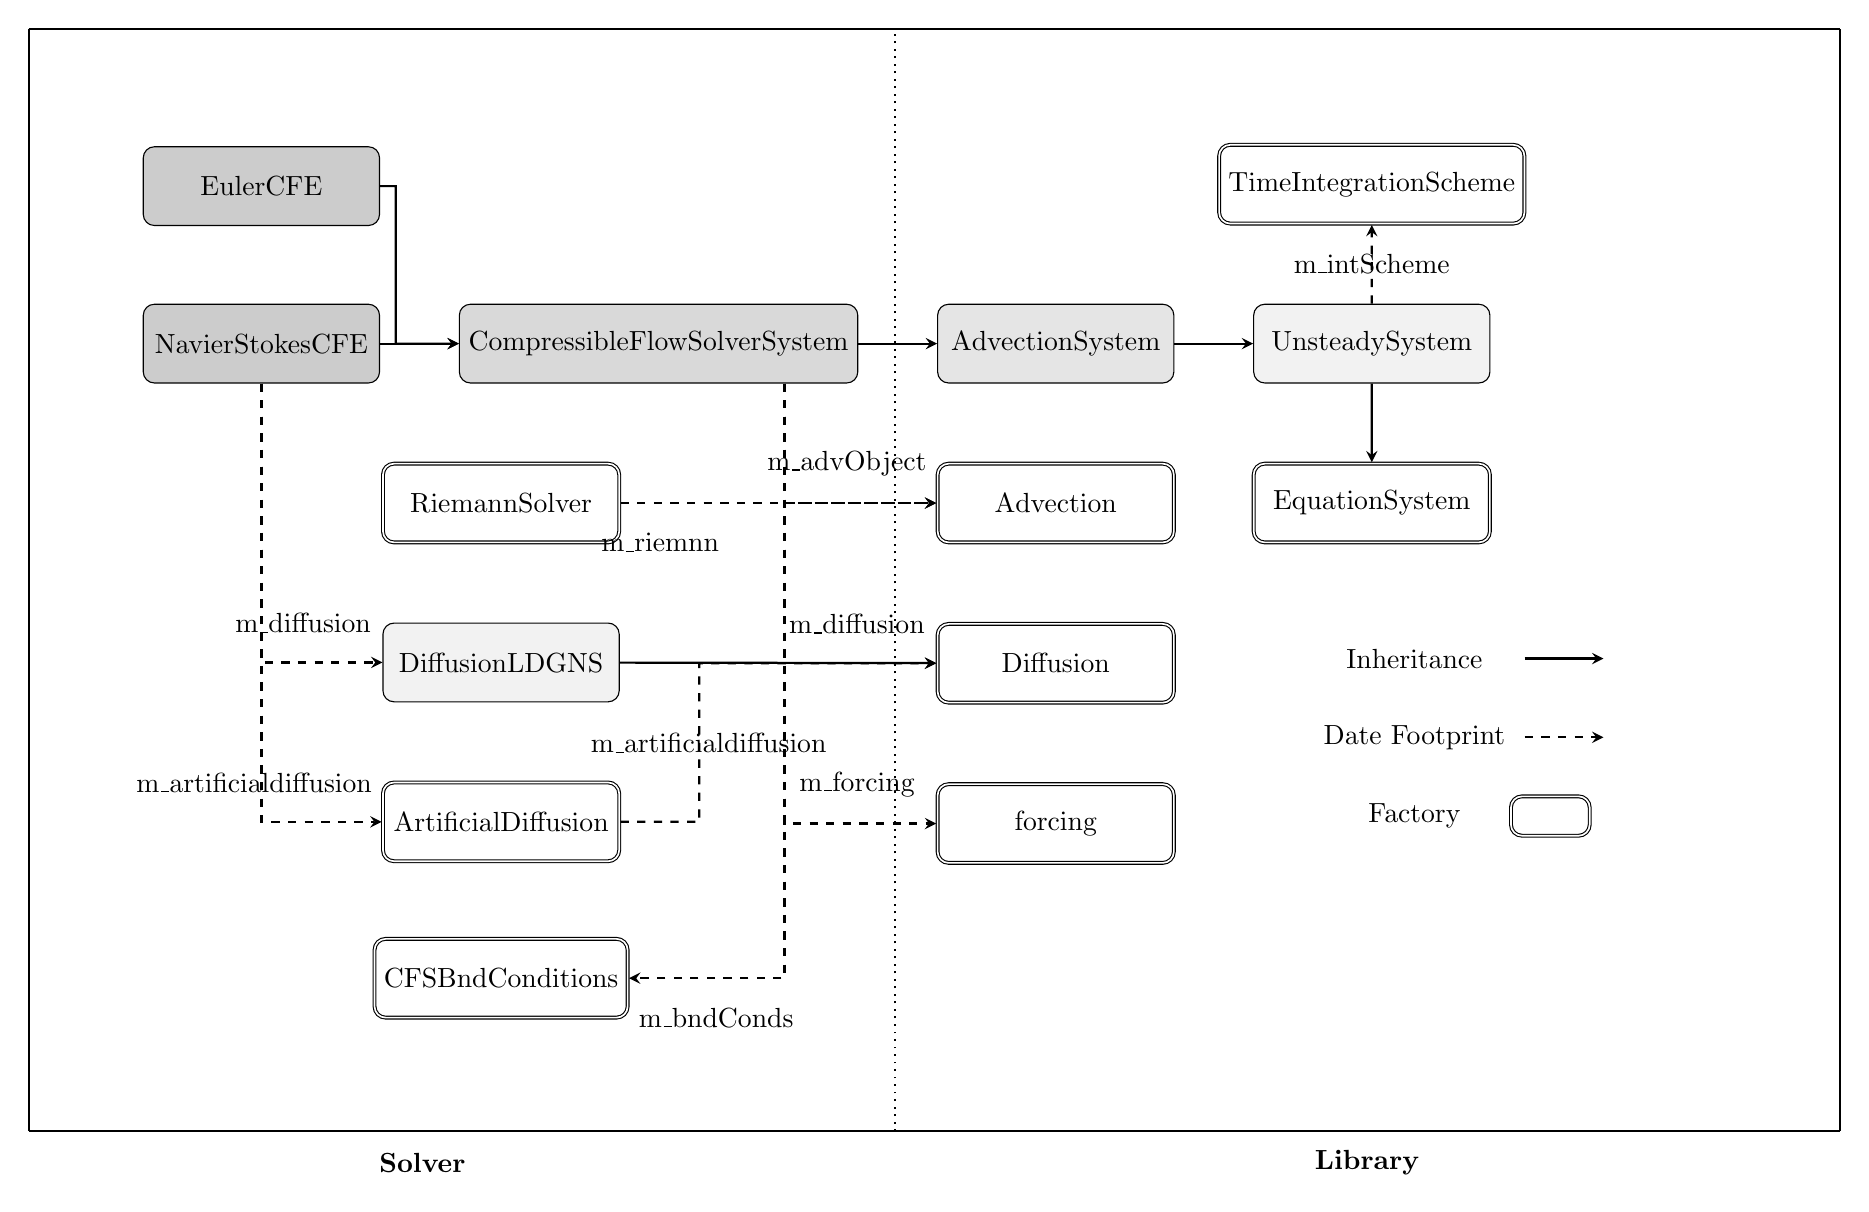
\begin{tikzpicture}[scale=0.2,node distance=1cm]
\node (A)
[rectangle,
rounded corners,
minimum width=3cm,
minimum height=1cm,
text centered,
draw=black,
fill=black!15]
{CompressibleFlowSolverSystem};
\node (B1)
[rectangle,
rounded corners,
minimum width=3cm,
minimum height=1cm,
text centered,
draw=black,
fill=black!20,
left = of A,
xshift=0cm,
yshift=2cm]
{EulerCFE};
\draw[arrow](B1)--($(B1.east)+(1,0)$)|-(A.west);
\node (B2)
[rectangle,
rounded corners,
minimum width=3cm,
minimum height=1cm,
text centered,
draw=black,
fill=black!20,
left = of A]
{NavierStokesCFE};
\draw[arrow](B2)--(A);
\node (A1)
[rectangle,
rounded corners,
minimum width=3cm,
minimum height=1cm,
text centered,
draw=black,
accepting,
fill=black!0,
below = of A,
xshift=-2cm,
yshift=0cm]
{RiemannSolver};
\node (A2)
[rectangle,
rounded corners,
minimum width=3cm,
minimum height=1cm,
text centered,
draw=black,
accepting,
fill=black!0,
below = of A1,
xshift=0cm,
yshift=-4cm]
{CFSBndConditions};
\draw[arrow1]($(A.south)+(8cm,0)$)|-(A2.east);
\node(text9)
[
minimum width=2cm,
minimum height=1cm,
text centered,
fill opacity=1,
right =of A2,
xshift=-1cm,
yshift=-0.5cm]
{m$\_$bndConds};
\node (A3)
[rectangle,
rounded corners,
minimum width=3cm,
minimum height=1cm,
text centered,
draw=black,
fill=black!5,
below = of A1,
xshift=0cm,
yshift=0cm]
{DiffusionLDGNS};
\draw[arrow1](B2.south)|-(A3.west);
\node(text4)
[
minimum width=2cm,
minimum height=1cm,
text centered,
fill opacity=1,
left =of A3,
xshift=1cm,
yshift=0.5cm]
{m$\_$diffusion};
\node (A4)
[rectangle,
rounded corners,
minimum width=3cm,
minimum height=1cm,
text centered,
draw=black,
accepting,
fill=black!0,
below = of A3,
xshift=0cm,
yshift=0cm]
{ArtificialDiffusion};
\draw[arrow1](B2.south)|-(A4.west);
\node(text5)
[
minimum width=2cm,
minimum height=1cm,
text centered,
fill opacity=1,
left =of A4,
xshift=1cm,
yshift=0.5cm]
{m$\_$artificialdiffusion};
\node(text11)
[
minimum width=2cm,
minimum height=1cm,
text centered,
fill opacity=1,
right =of A4,
xshift=-1.5cm,
yshift=1cm]
{m$\_$artificialdiffusion};
\node (C)
[rectangle,
rounded corners,
minimum width=3cm,
minimum height=1cm,
text centered,
draw=black,
fill=black!10,
right = of A]
{AdvectionSystem};
\draw[arrow](A)--(C);
\node (C1)
[rectangle,
rounded corners,
minimum width=3cm,
minimum height=1cm,
text centered,
draw=black,
accepting,
fill=black!0,
below = of C]
{Advection};
\draw[arrow1]($(A.south)+(8cm,0)$)|-(C1.west);
\node(text6)
[
minimum width=2cm,
minimum height=1cm,
text centered,
fill opacity=1,
left =of C1,
xshift=1cm,
yshift=0.5cm]
{m$\_$advObject};
\node(text7)
[
minimum width=2cm,
minimum height=1cm,
text centered,
fill opacity=1,
left =of C1,
xshift=-1.5cm,
yshift=-0.5cm]
{m$\_$riemnn};
\draw[arrow1](A1)--(C1);
\node (C2)
[rectangle,
rounded corners,
minimum width=3cm,
minimum height=1cm,
text centered,
draw=black,
accepting,
fill=black!0,
below = of C1]
{Diffusion};
\draw[arrow](A3)--(C2);
\draw[arrow1](A4)--($(A4.east)+(5cm,0)$)|-(C2);
\node(text8)
[
minimum width=2cm,
minimum height=1cm,
text centered,
fill opacity=1,
left =of C2,
xshift=1cm,
yshift=0.5cm]
{m$\_$diffusion};
\node (C3)
[rectangle,
rounded corners,
minimum width=3cm,
minimum height=1cm,
text centered,
draw=black,
accepting,
fill=black!0,
below = of C2]
{forcing};
\draw[arrow1]($(A.south)+(8cm,0)$)|-(C3.west);
\node(text9)
[
minimum width=2cm,
minimum height=1cm,
text centered,
fill opacity=1,
left =of C3,
xshift=1cm,
yshift=0.5cm]
{m$\_$forcing};
\node (D1)
[rectangle,
rounded corners,
minimum width=3cm,
minimum height=1cm,
text centered,
draw=black,
fill=black!5,
right = of C]
{UnsteadySystem};
\draw[arrow](C)--(D1);
\node (D2)
[rectangle,
rounded corners,
minimum width=3cm,
minimum height=1cm,
text centered,
draw=black,
accepting,
fill=black!0,
below = of D1]
{EquationSystem};
\draw[arrow](D1)--(D2);
\node (D3)
[rectangle,
rounded corners,
minimum width=3cm,
minimum height=1cm,
text centered,
draw=black,
accepting,
fill=black!0,
above= of D1]
{TimeIntegrationScheme};
\draw[arrow1](D1)--(D3);
\node(text12)
[
minimum width=2cm,
minimum height=1cm,
text centered,
fill opacity=1,
above =of D1,
xshift=0cm,
yshift=-1cm]
{m$\_$intScheme};
%\node (D4)
%[rectangle,
%rounded corners,
%minimum width=3cm,
%minimum height=1cm,
%text centered,
%draw=black,
%fill=black!0,
%below = of D2]
%{Explist};
%%\draw[arrow](D4)--(D5);
%\node(text1)
%[
%minimum width=2cm,
%minimum height=1cm,
%text centered,
%fill opacity=1,
%right =of D1]
%{m$\_$explist};
\draw[line width=0.25mm,  black](-40cm,-50cm)--(75cm,-50cm);
\draw[line width=0.25mm,   black](-40cm,20cm)--(75cm,20cm);
\draw[line width=0.25mm,   black](-40cm,-50cm)--(-40cm,20cm);
\draw[line width=0.25mm,   black](75cm,-50cm)--(75cm,20cm);
\draw [arrow](55,-20)--(60,-20);
\node (text15) at (48,-20) {Inheritance};
\draw [arrow1](55,-25)--(60,-25);
\node (text14) at (48,-25) {Date 
Footprint };
\node (text13) at (48,-30) {Factory};
\node (text14)
[rectangle,
rounded corners,
minimum width=1cm,
minimum height=0.5cm,
text centered,
draw=black,
accepting,
fill=black!0,
right= of text13,
xshift=-0.5cm,
yshift=0cm]
{};
\draw[line width=0.25mm,   black,dotted](15cm,-50cm)--(15cm,20cm);
\node (text10) at (-15,-52) {\textbf{Solver}};
\node (text11) at (45,-52) {\textbf{Library}};
% \draw[line width=0.2mm,  blue](-50cm,-50cm)--(80cm,-50cm);
% \draw[line width=0.2mm,  blue](-50cm,-50cm)--(80cm,-50cm);
\end{tikzpicture}

\end{document}

